\documentclass[11pt]{article}

\usepackage{alltt,fullpage,graphics,color,epsfig,amsmath, amssymb}
\usepackage{hyperref}
\usepackage{boxedminipage}
\usepackage[ruled,vlined]{algorithm2e}
\usepackage{amsmath}
\usepackage{commath}
\usepackage{graphicx}
\graphicspath{ {.} }
\newcommand{\floor}[1]{\lfloor #1 \rfloor}
\newcommand{\ceil}[1]{\lceil #1 \rceil}

\title{CS 512 Assignment 1}
\author{Daniel Campos}
\date{March 5th,2021}
\begin{document}

\maketitle
\section{Problem 1}
\subsection{List two differences between Frequent Pattern Growth algorithm and Apriori
algorithm
}
Apriori requires K+1 scans of the database while FPGrowth requires 2. The apriori algorithm is a breath first search while FPGrowth is divide and conquer.  Apriori requires a large amount of memory and FPGrowth does not. 
\subsection{Prove all nonempty subsets of a frequent itemset must also be frequent and prove the support of any nonempty subset s' of itemset s must be at least as large as the support of s.}
\subsubsection{Answer Prove all nonempty subsets of a frequent item list must be frequent}
\begin{enumerate}
    \item Let $S = {i_0, i_1,..., i_n}$ be a set of items.
    \item Let $R = {r_0, r_1, ...,r_m}$ be a set of records where each record $r_j$ is a set of items where $\forall k \in r_j$ $r_{jk} \in S$.
    \item Let $F = {i_0, i_1, ...,i_k}$ where each $\forall k \in F$ $F_k \in S$
    \item A frequent item set contains items where their occurrence is $>= minsup$ where minsup represents a minimum support threshold where only items that occur at or more than this threshold are in $F$. 
    \item Let $ss$ represent possible non empty subsets of $F$
    \item Since every possible $ss \in F$ all items in $ss$ occur $>= minsup$ and therefore all items $\in ss$ must all be frequent as well. 
    \item As a result, all non empty subsets of a frequent itemset must be frequent.
\end{enumerate}
\subsubsection{Prove any nonempty subset s must be at least as large as the support of s}
\begin{enumerate}
    \item Let $S = {i_0, i_1,..., i_n}$ be a set of items.
    \item Let $R = {r_0, r_1, ...,r_m}$ be a set of records where each record $r_j$ is a set of items where $\forall k \in r_j$ $r_{jk} \in S$.
    \item Given all non-empty subsets of $S$ where $s' = {i_1, i_k, ...}$ where $s' \in S$.
    \item Since the support of a itemset is driven by how often its items occur in $R$ the support of $S$ is that of its least common item. 
    \item Since all items $i_k \in ss$ are also in $S$ the support for $i_k \in s'$ > = support($S$).
    \item Since $\forall i_k \in s'> support(S)$ then we know $support(s') \ge support(s)$
    \item Thus all non-empty subsets $s'$ must be at least as large as the support of $S$
\end{enumerate}
\subsection{What problem might lift and $\chi^2$ have? Explain why Jaccard function is null-invariant}
Lift and $X^2$
\subsubsection{What problems do $Lift$ and $\chi^2$ have}
Neither deal way with datasets that have large amounts of null transaction for the variables being compared. In other words if we are studying the correlation between variable A and B and both A and B do not have a balanced occurrence(in other words $\neg A > A$ and $\neg B > B$ both $\chi^2$ and $Lift$ will not be good measures.
\subsubsection{Why is Jaccard function null-invariant}
The Jaccard function is null invariant because it is only looking at when variables occur and does not use information from where the variables do not occur. To build on our example from part a: Jaccard function looks at $A$ and $B$ and ignores $\neg A$ and $\neg B$. This makes Jaccard null-invariant.
\subsection{Under what circumstances will PrefixSpan also have poor performance}
Since the major cost in prefixspan is Constructing projected dbs and Suffixes are largely repeating, if the target records include a large quantity of unique items then storing the physical DB in memory can be prohibitive and require projections. In short when the transaction dataset is large and there are a large amount of prefixes(say items on amazon).  
\section{Problem 2: Apriori vs Frequent Pattern Growth}
\subsection{Present the intermediate results of the first three scans and the final derived frequent itemsets.}
\subsubsection{First Scan}
See results in table \ref{tab:1st}
\begin{table}[]
    \centering
    \begin{tabular}{|c|c|} \hline
        Itemset & Support \\ \hline
        A & 4 \\ \hline
        B & 3 \\ \hline
        C & 5 \\ \hline
        F & 4 \\ \hline
        M & 3 \\ \hline
        P & 3 \\ \hline
    \end{tabular}
    \caption{Apriori first scan}
    \label{tab:1st}
\end{table}
\subsubsection{Second Scan}
See results in table \ref{tab:2nd}
\begin{table}[]
    \centering
    \begin{tabular}{|c|c|} \hline
        Itemset & Support \\ \hline
        A,C & 4 \\ \hline
        A,M & 3 \\ \hline
        A,P & 3 \\ \hline
        C, F & 3 \\ \hline
        C, M & 3 \\ \hline
        C, P & 3 \\ \hline
    \end{tabular}
    \caption{Apriori second scan}
    \label{tab:2nd}
\end{table}
\subsubsection{Third Scan}
See results in table \ref{tab:3rd}
\begin{table}[]
    \centering
    \begin{tabular}{|c|c|} \hline
        Itemset & Support \\ \hline
        A, C, M & 3  \\ \hline
        A, C, P & 3  \\ \hline
    \end{tabular}
    \caption{Apriori third scan}
    \label{tab:3rd}
\end{table}
\subsubsection{Final derived frequent itemsets}
See results in table \ref{tab:final}
\begin{table}[]
    \centering
    \begin{tabular}{|c|c|} \hline
        Itemset & Support \\ \hline
        A & 4 \\ \hline
        B & 3 \\ \hline
        C & 5 \\ \hline
        F & 4 \\ \hline
        M & 3 \\ \hline
        P & 3 \\ \hline
        A,C & 4 \\ \hline
        A,M & 3 \\ \hline
        A,P & 3 \\ \hline
        C, F & 3 \\ \hline
        C, M & 3 \\ \hline
        C, P & 3 \\ \hline
        A, C, M & 3  \\ \hline
        A, C, P & 3  \\ \hline
    \end{tabular}
    \caption{Apriori Derived frequent itemsets}
    \label{tab:final}
\end{table}
\subsection{Frequent Pattern}
First off we go ahead and sort our items by frequency giving us the ordering: C(5), A(4), F(4), B(3), M(3), P(3).
Using the updated frequency sorted ordering the updated transactional database is found in table \ref{tab:sorted}.
\begin{table}[]
    \centering
    \begin{tabular}{|c|c|} \hline
        TID & ITEMS \\ \hline
        1 & {C, A, B, P} \\ \hline
        2 & {C, A, B, M} \\ \hline
        3 & {F, B} \\ \hline
        4 & {C, A, F, M, P} \\ \hline
        5 & {C, A, F, M, P} \\ \hline
        6 & {C, F} \\ \hline
    \end{tabular}
    \caption{FPGrowth updated and sorted transaction database}
    \label{tab:sorted}
\end{table}
Using this updated transaction database we create the pattern tree found in figure \ref{fig:fptree}.
\begin{figure}[]
\centering1
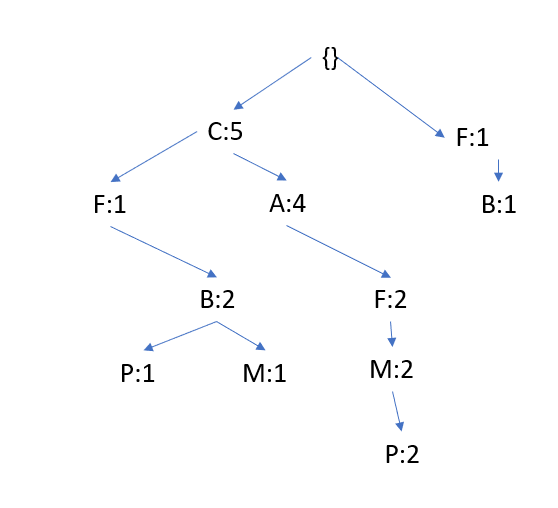
\includegraphics[width=8cm]{Assignments/Assignment1/FPtree.png}
\caption{Frequent Pattern Tree}
\label{fig:fptree}
\end{figure}
\subsection{Association rules}
Top 3 association rules and their confidence. \\
$M \rightarrow A = 1.0$ \\
$A \rightarrow C = 1.0$ \\
$P \rightarrow C = 1.0$ \\
\section{Problem 3: Frequent Pattern Mining Implementation}
\subsection{Data statistics}
\begin{table}[]
    \centering
    \resizebox{\textwidth}{!}{%
    \begin{tabular}{|c|c|} \hline
       Product Types  & 169  \\ \hline
       Transactions & 9835 \\ \hline
       Average Products per transactions & 4.41 \\ \hline 
       Top 5 most popular products  & Whole milk(2513), other vegetables(1903), rolls/buns(1809), soda(1715), yogurt(1372) \\ \hline
       Items with single purchase & baby food, sound storage medium  \\ \hline
    \end{tabular}}
    \caption{Grocery dataset statistics}
    \label{tab:stats}
\end{table}
\subsection{Results }
Using the minimum support values of 0.05 and confidence of 0.25 the top 10 frequent item sets:
\begin{enumerate}
    \item whole milk: 0.26
    \item other vegetables:0.19
    \item rolls/buns:0.184
    \item soda:0.174
    \item yogurt:0.140
    \item bottled water: 0.11
    \item root vegetables: 0.109
    \item tropical fruit: 0.11
    \item shopping bags: 0.10
    \item sausage:0.09
\end{enumerate}
Using the same thresholds the inferred rules are:
\begin{enumerate}
    \item (whole milk) $\rightarrow$ (other vegetables) : $0.29$
    \item (rolls/buns) $\rightarrow$ (whole milk) : $0.29$
    \item (other vegetables) $\rightarrow$ (whole milk) : $0.29$
    \item (yogurt) $\rightarrow$ (whole milk) : $0.40$
\end{enumerate}
\subsection{Contingency Table: Yogurt and Whole milk}
\begin{table}[]
    \centering
    \begin{tabular}{|c|c|c|c| } \hline
       Item & Yogurt & $\neg$ Yogurt & Total  \\ \hline
       Whole Milk & 551 & 1962 & 2513 \\ \hline
       $\neg$ Whole Milk & 821  & 6501&  7322\\ \hline 
       Total &1372 & 8463 &9835 \\ \hline
    \end{tabular}
    \caption{Caption}
    \label{tab:my_label}
\end{table}
\subsection{Interestingness using Lift}
Let A represent Whole milk and B represent yogurt. \\
\begin{equation}
lift(A,B) = \frac{c(A \rightarrow B)} {s(B)} = \frac{s(A \cup B)}{s(A)*s(B)} =  \frac{551/9836}{(1372/9835)*(2513/9835)}
\end{equation}
\begin{equation}
lift(A, B) = \frac{0.05601871}{(0.13950178)(0.25551601)} = \frac{0.05601871}{0.0356449382134978} = 1.5715754552433814 = 1.57
\end{equation}
Since the Lift of A and B is over one they are positively correlated. \\
\begin{equation}
lift(A,\neg B) = \frac{c(A \rightarrow B)} {s(B)} = \frac{s(A \cup B)}{s(A)*s(B)} =  \frac{1962/9836}{(8463/9835)*(2513/9835)} 
\end{equation}
\begin{equation}
lift(A, \neg B) =  \frac{0.1994713298088654}{(0.8604982206405694)(0.25551601)} = \frac{0.1994713298088654}{0.21987107195017794} = 0.9072195266054142 = 0.91
\end{equation}
Since the lift of A and $\neg B$ is under one they are negatively correlated.\\
\subsection{Run time}
My run times comparing our implementation in of Apriori in python vs FP-Growth(via pyfpgrowth)
\begin{table}[]
    \centering
    \begin{tabular}{|c|c|c|} \hline
       Transactions  & Apriori(ms) & FP-Growth(ms)  \\ \hline
       500 & 3.13e-5 & 1.58e-4 \\ \hline 
       1000 & 6.37e-5 & 5.98e-5 \\ \hline 
       2000 & 1.41e-4 & 7.90e-5 \\ \hline 
       5000 & 1.74e-4 & 6.35e-5\\ \hline 
       Full & 2.51e-4 & 1.09e-4 \\ \hline 
    \end{tabular}
    \caption{FP-Growth vs Apriori execution time}
    \label{tab:my_label}
\end{table}
\section{Problem 4: Sequential and Graph Pattern Mining}
\subsection{Sequential database}
\subsubsection{Projections }
for $\langle ab \rangle$ see table \ref{tab:ab}, for $\langle (ab) \rangle$ see table \ref{tab:(ab)}, for $\langle de \rangle$ see table \ref{tab:de}, for $\langle abc \rangle$ see table \ref{tab:abc}, for $\langle acb \rangle$ see table \ref{tab:acb},for $\langle abca \rangle$ see table \ref{tab:acba}    
\begin{table}[]
    \centering
    \begin{tabular}{|c|c|} \hline
       SID  & Sequence  \\ \hline
       1 & $\langle (_cf)(ac)b \rangle$ \\ \hline
       2 & $\langle (_)c(bc)ab(ce) \rangle$ \\ \hline
       3 & $\langle _(acf)acd \rangle$ \\ \hline
       4 & $\langle (_c)(ae) \rangle$ \\ \hline
       5 & $\langle (_d)df(ab) \rangle$\\ \hline
       6 & $\langle (_c)eab(cd)f(abd) \rangle$ \\ \hline
    \end{tabular}
    \caption{Projection for $\langle ab \rangle$}
    \label{tab:ab}
\end{table}
\begin{table}[]
    \centering
    \begin{tabular}{|c|c|} \hline
       SID  & Sequence  \\ \hline
       1 & $\langle  \rangle$ \\ \hline
       2 & $\langle c(bc)ab(ce) \rangle$ \\ \hline
       3 & $\langle  \rangle$ \\ \hline
       4 & $\langle (_c)(ae) \rangle$ \\ \hline
       5 & $\langle (_d)df(ab) \rangle$\\ \hline
       6 & $\langle (_c)eab(cd)f(abd) \rangle$ \\ \hline
    \end{tabular}
    \caption{Projection for $\langle (ab) \rangle$}
    \label{tab:(ab)}
\end{table}
\begin{table}[]
    \centering
    \begin{tabular}{|c|c|} \hline
       SID  & Sequence  \\ \hline
       1 & $\langle  \rangle$\\ \hline
       2 & $\langle  \rangle$ \\ \hline
       3 & $\langle _(af)acb(acf)acd \rangle$ \\ \hline
       4 & $\langle _(abc)(ae) \rangle$ \\ \hline
       5 & $\langle  \rangle$\\ \hline
       6 & $\langle  \rangle$ \\ \hline
    \end{tabular}
    \caption{Projection for $\langle de \rangle$}
    \label{tab:de}
\end{table}
\begin{table}[]
    \centering
    \begin{tabular}{|c|c|} \hline
       SID  & Sequence  \\ \hline
       1 & $\langle (_f)(ac)b \rangle$\\ \hline
       2 & $\langle _(bc)ab(ce) \rangle$ \\ \hline
       3 & $\langle (_f)acd \rangle$ \\ \hline
       4 & $\langle (_)(ae) \rangle$ \\ \hline
       5 & $\langle  \rangle$\\ \hline
       6 & $\langle eab(cd)f(abd) \rangle$ \\ \hline
    \end{tabular}
    \caption{Projection for $\langle abc\rangle$}
    \label{tab:abc}
\end{table}
\begin{table}[]
    \centering
    \begin{tabular}{|c|c|} \hline
       SID  & Sequence  \\ \hline
       1 & $\langle  \rangle$\\ \hline
       2 & $\langle (_c)ab(ce) \rangle$ \\ \hline
       3 & $\langle (acf)acd \rangle$ \\ \hline
       4 & $\langle  \rangle$ \\ \hline
       5 & $\langle (_d)df(ab) \rangle$\\ \hline
       6 & $\langle (cd)f(abd) \rangle$ \\ \hline
    \end{tabular}
    \caption{Projection for $\langle acb \rangle$}
    \label{tab:acb}
\end{table}
\begin{table}[]
    \centering
    \begin{tabular}{|c|c|} \hline
       SID  & Sequence  \\ \hline
       1 & $\langle _ \rangle$\\ \hline
       2 & $\langle _b(ce) \rangle$ \\ \hline
       3 & $\langle (_cf)acd \rangle$ \\ \hline
       4 & $\langle  \rangle$ \\ \hline
       5 & $\langle (_b) \rangle$\\ \hline
       6 & $\langle (_bd)  \rangle$ \\ \hline
    \end{tabular}
    \caption{Projection for $\langle acba\rangle$}
    \label{tab:acba}
\end{table}
\subsubsection{Sequential Patterns}
Sequential patterns where support = 3 and length $\ge 3$
ABC I guess
\subsection{Graph mining}
\subsubsection{Support}
P1 support is $\frac{4}{5}$ and is supported by G2, G3, G4, and G5. \\
P2 support is $\frac{3}{5}$ and is supported by G1, G2, and G5. \\
P3 support is $\frac{3}{5}$ and is supported by G1, G3 and G5.
\subsubsection{Apriori-based}
see figure \ref{fig:graph-apri}
\begin{figure}[]
\centering
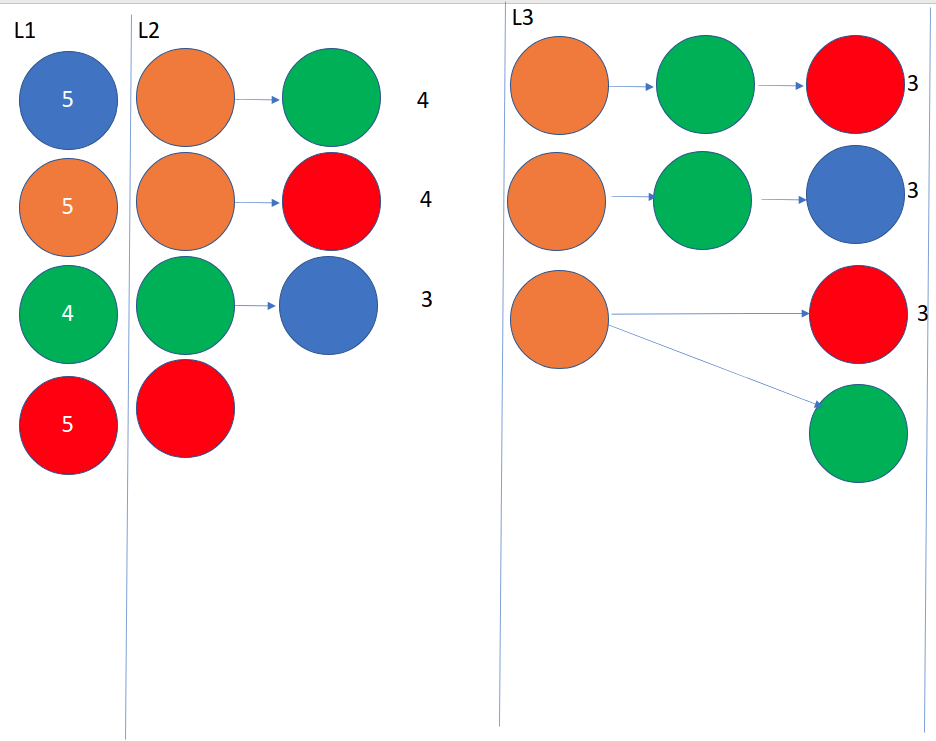
\includegraphics[width=8cm]{Assignments/Assignment1/graphapri.png}
\caption{Graph sequence apriori mining}
\label{fig:graph-apri}
\end{figure}
\section{Problem 5: SVM, RBF Kernel}
\subsection{Prove all eigenvalues are non negative}
We know from other work that every semdefinite matrix only has non negative eigenvalues. 
For a matrix to be semi-definite $x^TAx \ge 0$ for all $x \in \mathbf{R}^N $ . Since we know that $\text{k}(\bold{x}, \bold{x}') = \bold{x}^\top \bold{x}'$ to ensure semi-definite we ensure A > 0. Since A is the transform its always > 0. 
\subsection{Prove RBF Kernel is the sum of infinite polynomial kernels}
A kernel is any function in the form $K(x, y) = \langle \psi(x), \psi(y)\rangle$ where $\psi$ projects $x$ into a new vector space. \\
We are trying to prove that $\psi_{RBF}: \mathbf{R}^N \rightarrow \mathbf{R}^\infty$. \\
WLOG we set $\gamma = 1$
\begin{equation}
\begin{split}
K_{RBF}(x, y)  &= exp [-1 \abs{x -y}^2] \\
& = exp [-1 \langle x -y, x-y \rangle] \\
& = exp [-1 (\langle x, x -y \rangle - \langle y, x-y \rangle)] \\
& = exp [-1 (\langle x, x \rangle - \langle x,y \rangle -\langle y, x \rangle + \langle y,y \rangle)] \\
& = exp [-1 (\abs{x}^2 + \abs{y}^2 - 2 \langle x, y \rangle)] \\
& = exp[-1\abs{x}^2-1\abs{y}^2 ]exp[-1 -2 \langle x, y \rangle] \\ \\
c :&= exp[-1\abs{x}^2-1\abs{y}^2 ] \\ \\
K_{RBF}(x, y) &= c*e^{\lange x, y \rangle} \\
&= c \sum_{n=0}^{\infty} \frac{(\langle x, y \rangle)^n}{n!}  \text{via taylor expansion of $e^x$}  \\ 
&= c \sum_{n=0}^{\infty} \frac{K_{poly(n)}(x,y)}{n!}
\end{split}
\end{equation}
Thus we see that RBF is an infinite sum over poly kernels.
\subsection{Decision Boundary}
If we were to use a large $\gamma$ we would likely be able to separate the training data nearly perfectly. We would be over fitting to training but could likely produce results seen in figure \ref{fig:bound}
\begin{figure}[]
\centering
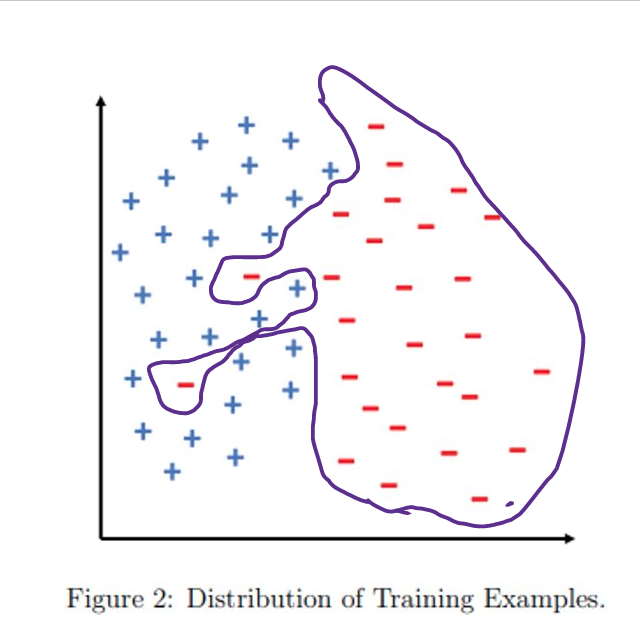
\includegraphics[width=8cm]{Assignments/Assignment1/decisionbound.png}
\caption{Decision Boundary using high $\gamma$}
\label{fig:bound}
\end{figure}
\subsection{Effect of large $\gamma$}
If we are to make the $\gamma$ infinitely large we will completely fit the SVM to the training data and overfit the model. Our training accuracy may reach 100\% but our transfer accuracy will suffer. This is because larger RBF kernel bandwidths(which are smaller $\gamma$ values produce a smoother feature space mapping. As we scale our $\gamma$ value we produce a less smooth kernel which will allow us to learn harder decision boundaries but will overfit to the decision boundary of the training corpus. 
\section{Problem 6:Feature Selection}
\subsection{Classification Results}
On the test portion accuracy:0.68, precision:0.76, recall:0.38, F1 score:0.51. More detailed breakdown can be found in table \ref{tab:Accuracy}
\begin{table}[]
    \centering
    \begin{tabular}{|c|c|c|} \hline
       Reference Label  & Predicted 0 & Predict 1   \\ \hline
       0 & 60 & 6 \\ \hline
       1 & 31 & 19 \\ \hline
    \end{tabular}
    \caption{SVM}
    \label{tab:Accuracy}
\end{table}
\subsection{Fisher Score Feature Selection}
Using Fisher Score calculation and a threshold of $\ge$ 1 we find that only columns [8, 11, 18, 26] pass the threshold. We then remove all the other indexes and retrain our svm. Performance on train goes from 0.81 to 0.94 and performance on test goes from 0.68 to 0.84!  On the test portion accuracy:0.84, precision:0.88, recall:0.72, F1 score:0.79 . More detailed breakdown can be found in table \ref{tab:Accuracy2}
\begin{table}[]
    \centering
    \begin{tabular}{|c|c|c|} \hline
       Reference Label  & Predicted 0 & Predict 1   \\ \hline
       0 & 61 & 5 \\ \hline
       1 & 36 & 14 \\ \hline
    \end{tabular}
    \caption{Fisher Score Augmented SVM}
    \label{tab:Accuracy2}
\end{table}
\section{Problem 7:Self Training}
Using self training we first train an svm based on the regular training corpus(non fisher score adjusted). Then, we label the unlabeled corpus and only keep data where confidence is $\ge$ 0.6. By that we mean there is over a 0.6 difference between the confidence scores and we set the winning label to the self-trained label. Using this threshold of training we include 322 inferred label samples in our training data. \\
Using this amplified training data we find performance improvements on non Fisher-score optimized models and fisher score optimized models. Without using fisher-score optimization the introduction of self-trained data improves F1 score from 0.51 to 0.55, recall goes from 0.38 to 0.42, precision goes from 0.76 to 0.78. More details available on self training model performance are available in table \ref{tab:Accuracy3}. Using fisher score optimization the amplified training data improves F1 from 0.79 to 0.80, recall goes from 0.72 to 0.74, precision goes from 0.88 to 0.86. More details about fisher+self training model performance are available in table \ref{tab:Accuracy4}
\begin{table}[]
    \centering
    \begin{tabular}{|c|c|c|} \hline
       Reference Label  & Predicted 0 & Predict 1   \\ \hline
       0 & 60 & 6 \\ \hline
       1 & 29 & 21 \\ \hline
    \end{tabular}
    \caption{Self-Training Augmented SVM}
    \label{tab:Accuracy3}
\end{table}
\begin{table}[]
    \centering
    \begin{tabular}{|c|c|c|} \hline
       Reference Label  & Predicted 0 & Predict 1   \\ \hline
       0 & 60 & 6 \\ \hline
       1 & 13 & 37 \\ \hline
    \end{tabular}
    \caption{Fisher Score and Self Training Augmented SVM}
    \label{tab:Accuracy4}
\end{table}
\section{Random Walk with Restart}
\subsection{Capture multiple weighted relationships}
\end{document}